\documentclass[a4paper, 12pt]{article}
\usepackage[T2A]{fontenc}
\usepackage[utf8]{inputenc}
\usepackage[english,russian]{babel}
\usepackage{amsmath, amsfonts, amssymb, amsthm, mathtools, misccorr, indentfirst, multirow}
\usepackage{wrapfig}
\usepackage{graphicx}
\usepackage{subfig}
\usepackage{enumitem}
\usepackage{adjustbox}
\usepackage{pgfplots}

\usepackage{geometry}
\geometry{top=20mm}
\geometry{bottom=20mm}
\geometry{left=20mm}
\geometry{right=20mm}
\newcommand{\angstrom}{\textup{\AA}}
\begin{document}
	\begin{titlepage}
		\begin{center}
		МИНИСТЕРСТВО ОБРАЗОВАНИЯ И НАУКИ РОССИЙСКОЙ ФЕДЕРАЦИИ\\
		\footnotesize{Московский физико-технический институт}\\
		\footnotesize{(государственный университет)}\\
		\vfill
		{\LARGE
		\textbf{Оптика лазерных пучков}\\
		}
		\vspace{1cm}
		Лабораторная работа по курсу\\
		фотоника
		\vfill
		\begin{flushright}
			Выполнил: студенты 654гр.\\
			Нехаев А.С.\\
		\end{flushright}
		\vfill
		г. Долгопрудный\\
		\the\year\:год
		\end{center}
	\end{titlepage}
	\newpage
	\section{Цели и задачи исследования}
	\begin{enumerate}
		\item Освоить методику расчёта параметров резонатора, образованного гауссовыми оптическими элементами.
		\item Определить экспериментально модовый состав лазерного излучения.
	\end{enumerate}
	\section{Практическая часть}
	\begin{enumerate}
		\item Проведем измерения распределения интенсивности лазерного пучка с линзой в поперечном сечении. Результат измерения отобразим на графике
		\begin{figure}[!htb]
			\centering
			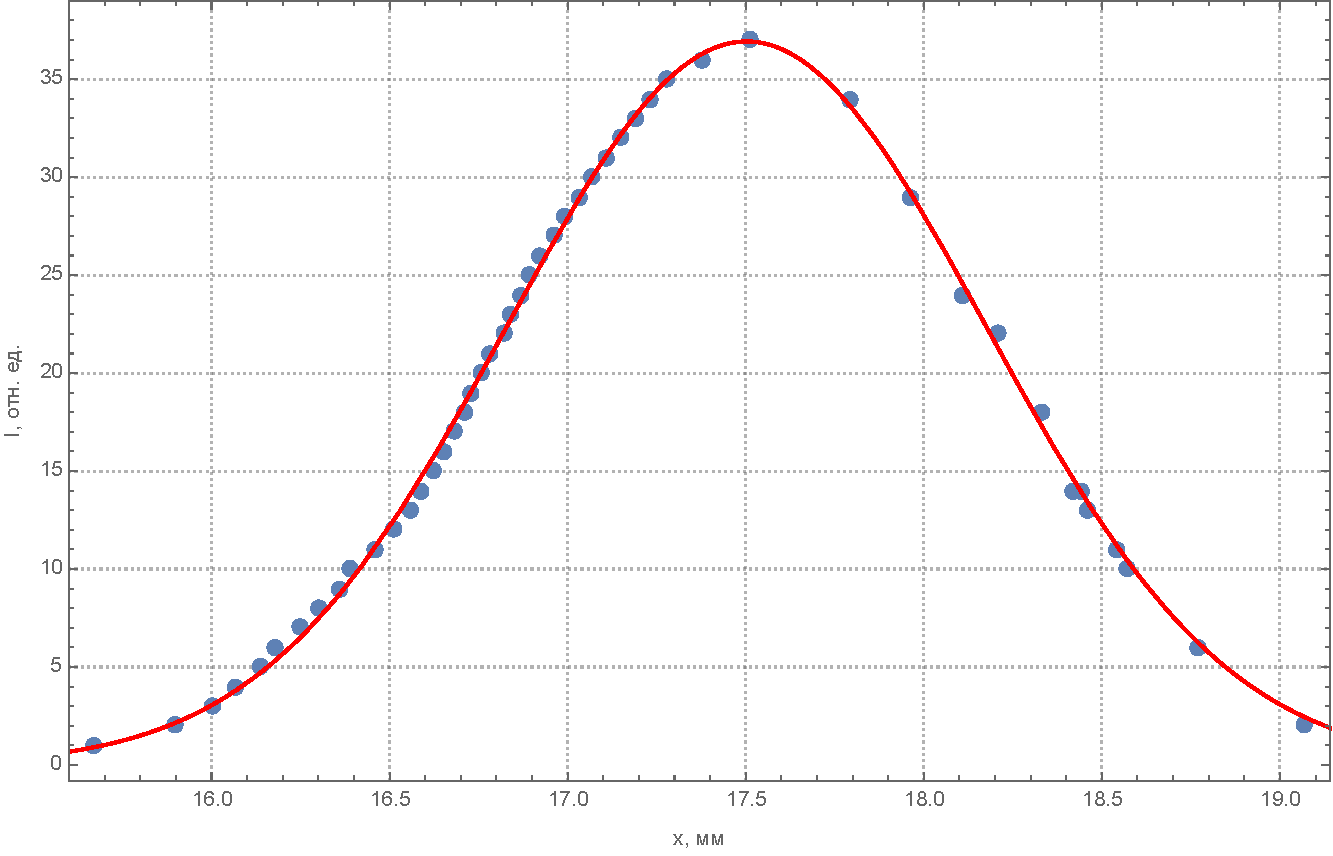
\includegraphics[width=\textwidth]{graph.pdf}
			\caption{Поперечная структура лазерного пучка с линзой}
		\end{figure}
		\item Определим характерную полуширину пучка $\sigma=1.58$ мм.
	\end{enumerate}
	\section{Вывод}
	В ходе работы была определена характерная полуширина лазерного пучка с линзой. Также были освоены основы теории лазерных резонаторов и методы анализа лазерных пучков.
\end{document}